\documentclass[12pt]{extarticle}

\usepackage{datetime}
\usepackage{wrapfig}
\usepackage{enumerate}
\usepackage{float}
\usepackage{graphicx}
\usepackage{caption}
\usepackage[acronym]{glossaries}
\usepackage{glossaries-polyglossia}
\usepackage[nottoc]{tocbibind}
\usepackage{siunitx}
\usepackage{subcaption}
\usepackage{geometry}
\usepackage{fancyhdr}
\usepackage{cite}
\usepackage{subfiles}
\usepackage{amsmath}
\usepackage{array,tabularx}
\usepackage{chngcntr}
\usepackage{afterpage}
\usepackage{ulem}
\usepackage{polyglossia}
\usepackage{fontspec}
\usepackage{hyperref}
\usepackage{dirtytalk}
\usepackage{algorithm2e}
\usepackage{enumitem,amssymb}
\usepackage{pifont}
\usepackage{amsmath}
\usepackage{listings}
\usepackage{xcolor}
\usepackage{formal-grammar}
\usepackage{varwidth}
\usepackage{fmtcount}
\usepackage{tikz}
\usepackage{tikzpeople}
\usepackage{array}
\usepackage[framemethod=tikz]{mdframed} % Allows defining custom boxed/framed environments
\usepackage{cleveref}
\usepackage{epigraph}
\usepackage{microtype}
\usepackage{dirtytalk}

\usetikzlibrary{trees}
\usetikzlibrary{fit}
\usetikzlibrary{shapes}
\usetikzlibrary{arrows.meta, positioning, shadows}
\usetikzlibrary{chains,shapes.multipart}
\usetikzlibrary{external}
\usetikzlibrary{matrix}

\tikzstyle{rect} = [rectangle,fill=white, text centered]
\tikzstyle{database} = [draw, cylinder, shape border rotate = 90, aspect = 0.2]
\tikzstyle{thick-arrow} = [->, thick]
\tikzstyle{arrow} = [thick,->,>=stealth]
\tikzstyle{arrow-small} = [->,>=stealth]
\tikzstyle{simple-rect} = [rectangle, text centered, draw = black, inner sep=4mm]

\tikzset{
    doc/.style={draw, minimum height=4em, minimum width=3em, 
                fill=white, 
                double copy shadow={shadow xshift=4pt, 
                             shadow yshift=4pt, fill=white, draw}}
}

\tikzset{
    dcs/.style = {double copy shadow},
}

\setmainfont[Mapping=tex-text]{CMU Serif}
\setsansfont[Mapping=tex-text]{CMU Sans Serif}
\setmonofont{CMU Typewriter Text}

\setotherlanguage[variant=british]{english}
\setmainlanguage[]{greek}

\hypersetup{
    colorlinks=true,
    filecolor=magenta,      
    urlcolor=blue,
}

\hypersetup{linkcolor=black}

\newcommand{\src}[1]{\texttt{#1}}

\lstset{basicstyle=\footnotesize\ttfamily,breaklines=true, captionpos=b}

% MD Frames

\mdfdefinestyle{commandline}{
	leftmargin=10pt,
	rightmargin=10pt,
	innerleftmargin=15pt,
	middlelinecolor=black!50!white,
	middlelinewidth=2pt,
	frametitlerule=false,
	backgroundcolor=black!5!white,
	frametitle={LLM Output},
	frametitlefont={\normalfont\sffamily\color{white}\hspace{-1em}},
	frametitlebackgroundcolor=black!50!white,
	nobreak,
	singleextra={%
    }
}

% Define a custom environment for command-line snapshots
\newenvironment{commandline}{
	\medskip
	\begin{mdframed}[style=commandline]
}{
	\end{mdframed}
	\medskip
}

\mdfdefinestyle{warning}{
	topline=false, bottomline=false,
	leftline=false, rightline=false,
	nobreak,
	singleextra={%
		\draw(P-|O)++(-0.5em,0)node(tmp1){};
		\draw(P-|O)++(0.5em,0)node(tmp2){};
		\fill[black,rotate around={45:(P-|O)}](tmp1)rectangle(tmp2);
		\node at(P-|O){\color{white}\scriptsize\bf ?};
		\draw[very thick](P-|O)++(0,-1em)--(O);%--(O-|P);
	}
}

% Define a custom environment for warning text
\newenvironment{prompt}[1][Prompt:]{ % Set the default warning to "Warning:"
	\medskip
	\begin{mdframed}[style=warning]
		\noindent{\textbf{#1}}
}{
	\end{mdframed}
}

\renewcommand{\lstlistingname}{Καταχώριση}


\title{Αυτόματη διάγνωση ασθενειών με χρήση Μεγάλων Γλωσσικών Μοντέλων και Answer Set Programming}
\author{Ιωάννα Γέμου\thanks{Τμήμα Ηλεκτρολόγων Μηχανικών και Τεχνολογίας Υπολογιστών, Πανεπιστήμιο Πατρών} \\ \src{ioannagemou@upnet.gr} \and Ευάγγελος Λάμπρου\footnotemark[1] \\ \src{e.lamprou@upnet.gr}}

\begin{document}

\maketitle
\tableofcontents
\newpage
\section{Περίληψη}
Η ανάπτυξη αυτόματων συστημάτων πρόβλεψης ασθενειών έχει κρίσιμη σημασία για τη βελτίωση της ανθρώπινης υγείας και την υποστήριξη των ιατρών στην ακριβή διάγνωση και αντιμετώπιση των ασθενειών. Η ακριβής διάγνωση είναι κρίσιμη για την έγκαιρη αντιμετώπιση και αποτελεσματική θεραπεία, ενώ μπορεί επίσης να συμβάλει στην αποφυγή περαιτέρω επιπλοκών και επιβαρυντικών ιατρικών διαδικασιών. 
Η συμβολική τεχνητή νοημοσύνη έχει ξαναεφαρμοστεί στο πεδίο της ιατρικής \cite{Alviano_2020}. Ωστόσο,
εφαρμογή πάντα ήταν περιορισμένη λόγω των σύνθετων βάσεων γνώσης που θα έπρεπε να αναπτυχθούν για τη λειτουργία 
αυτών των συστημάτων.
Η προτεινόμενη μέθοδος, η οποία συνδυάζει τα Large Language Models και το Answer Set Programming (ASP), αποτελεί ένα ισχυρό εργαλείο, καθώς παρέχει ένα αξιόπιστο και γρήγορο μέσο δημιουργίας μιας βάσης γνώσης η οποία 
στη συνέχεια μπορεί να χρησιμοποιηθεί για την πρόβλεψη ασθενειών.



Η καινοτομία της προτεινόμενης μεθόδου έγκειται στον συνδυασμό των δύο μεθοδολογιών. Τα Large Language Models μπορούν να κωδικοποιήσουν την ιατρική βιβλιογραφία 
σε κώδικα ASP με αξιοσημείωτη ακρίβεια και σύνθετη κατανόηση, ενώ το ASP παρέχει τον συλλογισμό και την επεξηγηματικότητά του. Ο συνδυασμός αυτών των δύο προσεγγίσεων επιτρέπει την ανάπτυξη ενός ισχυρού συστήματος πρόβλεψης ασθενειών που συνδυάζει την \textbf{ακρίβεια και την ευφυΐα των γλωσσικών μοντέλων} με την \textbf{επεξηγηματικότητα και την αποδοτικότητα του Answer Set Programming}.

Η μέθοδός μας φαίνεται να έχει υποσχόμενα αποτελέσματα πάνω στο σύνολο των δεδομένων ασθενών, στο οποίο
την εφαρμόσαμε.





\section{Ανασκόπηση Βιβλιογραφίας}

\subsection{Large Language Models}

Τα μεγάλα γλωσσικά μοντέλα \cite{zhao2023survey} είναι προηγμένα υπολογιστικά μοντέλα που έχουν σχεδιαστεί για να κατανοούν και να δημιουργούν ανθρώπινη γλώσσα. Αυτά τα μοντέλα, που αναπτύχθηκαν χρησιμοποιώντας εξελιγμένες τεχνικές μηχανικής μάθησης, έχουν τη δυνατότητα να επεξεργάζονται και να δημιουργούν κείμενο με τρόπο που μοιάζει πολύ με τα πρότυπα ανθρώπινης γλώσσας.

Μεγάλα γλωσσικά μοντέλα, όπως η αρχιτεκτονική \textit{GPT-4} \cite{openai2023gpt4}, εκπαιδεύονται σε τεράστιες ποσότητες δεδομένων κειμένου, γεγονός που τους επιτρέπει να αποκτούν γνώση σε διάφορους τομείς και θέματα. Αυτά τα μοντέλα χρησιμοποιούν αλγόριθμους βαθιάς μάθησης (deep learning) \cite{Sarker2021} και ειδικά δίκτυα μετασχηματιστών (transformer networks) \cite{Dosovitskiy2020}, για την ανάλυση και την κατανόηση των σχέσεων μεταξύ λέξεων, φράσεων και προτάσεων. Καταγράφοντας μοτίβα και δομές στα δεδομένα εκπαίδευσης, αυτά τα μοντέλα μπορούν να δημιουργήσουν συνεκτικές και συναφείς
απαντήσεις με βάση δοθέντα prompts.

Tα μοντέλα ονομάζονται \say{μεγάλα} επειδή έχουν δισεκατομμύρια παραμέτρους που διαμορφώνουν τις αποκρίσεις τους. Η βασική προϋπόθεση ενός γλωσσικού μοντέλου είναι η ικανότητά του να προβλέπει την επόμενη λέξη (που ονομάζεται token) με βάση το κείμενο που έχει παρατηρήσει μέχρι τώρα, δηλαδή σύμφωνα με τα συμφραζόμενα.


Τα μεγάλα γλωσσικά μοντέλα διαθέτουν την αξιοσημείωτη ικανότητα να μετασχηματίζουν κείμενο από τη μια μορφή στην άλλη, καθιστώντας τα ισχυρά εργαλεία για διάφορες εργασίες επεξεργασίας γλώσσας. 
Πάνω σε αυτό το χαρακτηριστικό τους, βασίζεται και η ιδέα αυτής της εργασίας, αφού ένα πολύ σημαντικό κομμάτι που πραγματευόμαστε είναι η κατάλληλη κωδικοποίηση της ιατρικής βιβλιογραφίας.
Παρακάτω αναφέρουμε κάποια παραδείγματα χρήσης των μεγάλων γλωσσικών μοντέλων \cite{Paranjape2023}: 

\begin{itemize}
    \item Δημιουργία κειμένου που είναι συναφές και συνεκτικό με βάση τα συμφραζόμενα
    \item Μετάφραση Γλώσσας
    \item Σύνοψη / Περίληψη Κειμένου
    \item  Απάντηση σε ερωτήσεις
    \item Παραγωγή κειμένου με βάση συγκεκριμένων κανόνων που τους παρέχονται
\end{itemize}

Ο θεμέλιος λίθος των Μεγάλων Γλωσσικών μοντέλων είναι οι \textbf{transformers}.
Οι transformers \cite{Vaswani2017} επί του παρόντος θεωρούνται μία από τις πιο προηγμένες και ισχυρές κατηγορίες μοντέλων. Συνέβαλαν καθοριστικά στην επίτευξη σημαντικών ανακαλύψεων στη μηχανική μάθηση, με αποτέλεσμα ορισμένοι να τους αναφέρουν ως \say{transformers AI}. Aυτά τα μοντέλα οδηγούν σε μια θεμελιώδη αλλαγή στον τομέα της τεχνητής νοημοσύνης \cite{Bommasani2021}.
To σχήμα \ref{fig:transformers} απεικονίζει τη δομή του transformer, ο οποίος περιλαμβάνει δύο διακριτά μέρη, την κωδικοποίηση και την αποκωδικοποίηση.

\begin{figure}[htb]
    \centering
    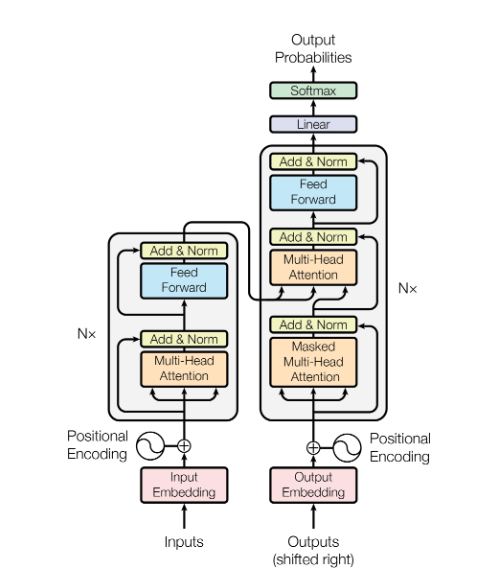
\includegraphics[width=0.7\textwidth]{assets/transformers_architecture.png}
    \caption{Αρχιτεκτονική του μοντέλου transformer \cite{Vaswani2017}.}
    \label{fig:transformers}
\end{figure}

\subsubsection{Inputs and Input Embeddings}

Tο θεμελιώδες συστατικό του
transformer, ο μηχανισμός \say{προσοχής} είναι εμπνευσμένος από την έννοια της συνειδητής προσοχής στους ζωντανούς οργανισμούς \cite{Vaswani2017}.
Αυτός ο μηχανισμός επιτρέπει στο δίκτυο να αποδίδει μεγαλύτερη σημασία σε κρίσιμα μέρη των δεδομένων και λιγότερη σημασία σε αυτά που είναι λιγότερο σχετικά. Αν και η απλούστερη μορφή αυτής της συνάρτησης είναι ένα σταθμισμένο άθροισμα των τιμών εισόδου, ο μηχανισμός προσοχής στον μετασχηματιστή είναι πιο περίπλοκος και περιλαμβάνει πολλαπλούς μετασχηματισμούς για τον υπολογισμό των βαρών προσοχής μεταξύ διαφορετικών τμημάτων της εισόδου.




















Τα τμήματα εισόδου από τον χρήστη είναι είσοδοι για τα μοντέλα μηχανικής μάθησης. Ωστόσο, τα μοντέλα κατανοούν μόνο αριθμούς, όχι κείμενο, επομένως αυτές οι είσοδοι πρέπει να μετατραπούν σε μια αριθμητική μορφή που ονομάζεται \textbf{input embeddings}. Tα input embeddings αντιπροσωπεύουν λέξεις ως αριθμούς, τους οποίους μπορούν στη συνέχεια να επεξεργαστούν τα μοντέλα μηχανικής μάθησης. Τα embeddings είναι σαν ένα λεξικό, το οποίο βοηθά το μοντέλο να κατανοήσει τη σημασία των λέξεων, μέσω της τοποθέτησής τους σε έναν μαθηματικό χώρο όπου παρόμοιες λέξεις βρίσκονται η μία κοντά στην άλλη. Κατά τη διάρκεια της εκπαίδευσης, το μοντέλο μαθαίνει πώς να δημιουργεί τα embeddings, έτσι ώστε παρόμοια διανύσματα να αντιπροσωπεύουν λέξεις με παρόμοια σημασία.

\subsubsection{Positional Encodings}

Στην επεξεργασία φυσικής γλώσσας, η σειρά των λέξεων σε μια πρόταση είναι κρίσιμη για τον προσδιορισμό του νοήματος της πρότασης. Ωστόσο, τα παραδοσιακά μοντέλα μηχανικής μάθησης, όπως τα νευρωνικά δίκτυα, δεν κατανοούν εγγενώς τη σειρά των εισόδων. Για την αντιμετώπιση αυτής της πρόκλησης, η κωδικοποίηση θέσης μπορεί να χρησιμοποιηθεί για την κωδικοποίηση της θέσης κάθε λέξης σε μία πρόταση. Η κωδικοποίηση αυτή τροφοδοτείται στο μοντέλο Transformer, μαζί με τα input embeddings. Με την ενσωμάτωση της κωδικοποίησης θέσης στην αρχιτεκτονική του Transformer, το μοντέλο μπορεί να κατανοήσει πιο αποτελεσματικά τη σειρά των λέξεων σε μια πρόταση και να δημιουργήσει γραμματικά σωστά και σημασιολογικά νόημα.
Το \say{γραμματικά σωστό} αποτέλεσμα μπορεί να σημαίνει και την παραγωγή κώδικα ο οποίος είναι 
σύμφωνος με τους κάνόνες μιας γλώσσας προγραμματισμού. 

\subsubsection{Encoder}

Ο κωδικοποιητής (encoder) είναι μέρος του νευρωνικού δικτύου που επεξεργάζεται το κείμενο εισόδου και δημιουργεί μια σειρά από κρυφές καταστάσεις που καταγράφουν το νόημα του κειμένου. Ο κωδικοποιητής διαμορφώνει πρώτα το κείμενο εισόδου σε μια ακολουθία tokens, π.χ. μεμονωμένες λέξεις.

\subsubsection{Decoder}
Ο αποκωδικοποιητής (decoder) είναι μέρος του μοντέλου που δημιουργεί την ακολουθία εξόδου με βάση την κωδικοποιημένη ακολουθία εισόδου. Κατά τη διάρκεια της εκπαίδευσης, ο αποκωδικοποιητής μαθαίνει πώς να \say{μαντεύει} την επόμενη λέξη κοιτάζοντας τις λέξεις πριν από αυτήν. Για παράδειγμα, ο αποκωδικοποιητής σε \textit{GPT} δημιουργεί κείμενο φυσικής γλώσσας με βάση την ακολουθία εισόδου και το περιβάλλον που μαθαίνει ο κωδικοποιητής. Στους transformers χρησιμοποιούνται πολλαπλά στρώματα αποκωδικοποιητών.

\subsection{Δυσκολίες στην εφαρμογή των LLMs}

Τα μεγάλα γλωσσικά μοντέλα δεν είναι αλάνθαστα \cite{Raj2023}, \cite{Ruis2023}. Μπορούν περιστασιακά να παράγουν λανθασμένες ή μεροληπτικές απαντήσεις, αντανακλώντας τις προκαταλήψεις που υπάρχουν στα δεδομένα εκπαίδευσης. Καταβάλλονται προσπάθειες για τον μετριασμό αυτών των ζητημάτων μέσω τεχνικών προεπεξεργασίας δεδομένων και fine-tuning.

Συνολικά, τα μεγάλα γλωσσικά μοντέλα έχουν επιδείξει τεράστιες δυνατότητες σε ένα ευρύ φάσμα εφαρμογών, συμπεριλαμβανομένης της κατανόησης φυσικής γλώσσας, της δημιουργίας περιεχομένου και της αλληλεπίδρασης ανθρώπου-υπολογιστή. Η συνεχής έρευνα και ανάπτυξη σε αυτόν τον τομέα υπόσχεται περαιτέρω ενίσχυση αυτών των μοντέλων και των εφαρμογών τους σε διάφορους τομείς, συμβάλλοντας στην πρόοδο των τεχνολογιών γλωσσικής επεξεργασίας και επικοινωνίας.

\subsection{Answer Set Programming}
To Answer Set Programming (ASP) \cite{Eiter2009} είναι μια δηλωτική μέθοδος επίλυσης προβλημάτων που βασίζεται στον Λογικό Προγραμματισμό και τη Μη Μονοτονική Συλλογιστική.  
Στην εργασία \cite{Gelfond2000} επισημοποιήθηκε αρχικά η σημασιολογία των σταθερών μοντέλων και η βασική γλώσσα του ASP.

Ο προγραμματισμός με χρήση αυτής της προσέγγισης γίνεται σε μια οικογένεια γλωσσών που ονομάζεται ορισμένες φορές \textit{AnsProlog} \cite{Gelfond2002}.

Η ιδέα πίσω από το ASP είναι να μοντελοποιηθεί ένα πρόβλημα ως ένα σύνολο κανόνων και δεδομένων, και στη συνέχεια να χρησιμοποιηθεί ένας επίλυτης για να βρεθεί μια λύση για το πρόβλημα. Οι λύσεις παριστάνονται από σταθερά μοντέλα ή σύνολα απαντήσεων. Οι κανόνες, τα δεδομένα και οι περιορισμοί που περιγράφουν το πρόβλημα αποτελούν τα στοιχεία του προγράμματος. Στη συνέχεια, το πρόγραμμα δίνεται σε έναν επίλυτη που θα βρει μία ή περισσότερες λύσεις. 

Στον παραδοσιακό προγραμματισμό, η μετάβαση από ένα πρόβλημα σε μια λύση προϋποθέτει την απόλυτη κατανόηση του δεδομένου προβλήματος από τον προγραμματιστή, και έπειτα την παραγωγή ενός προγράμματος, στο οποίο όταν δοθεί ένα instance του προβλήματος θα παράγει το σωστό αποτέλεσμα, τα οποίο στη συνέχεια θα ερμηνευτεί ως λύση.

Στο ASP, η μετάβαση από τη δήλωση προβλήματος σε ένα σύνολο λύσεων περιλαμβάνει τα ακόλουθα βήματα \cite{Gebser2013}
(εικόνα \ref{fig:asp-solving}):

\begin{figure}[htb]
    \begin{center}
\begin{tikzpicture}[node distance=4cm]
        \node [simple-rect] (problem)  at (0,0) {Problem};
        \node [simple-rect, below of=problem] (program) {Program};
        
        \node [simple-rect, right of=program] (grounder) {Grounder};
        \node [simple-rect, right of=grounder] (solver) {Solver};
        
        \node [simple-rect, right of=solver] (stable-models) {Stable Models};
        
        \node [simple-rect, above of=stable-models] (solution) {Solution};

        \draw [arrow] (problem) -- node[right] {\textbf{Modelling}} (program);
        \draw [arrow] (stable-models) -- node[left] {Interpreting} (solution);

        \draw [arrow-small] (program) -- node[above] {} (grounder);
        \draw [arrow-small] (grounder) -- node[above] {\footnotesize Grounding} (solver);
        \draw [arrow-small] (solver) -- node[above] {} (stable-models);

        \node[draw, dotted, fit=(grounder) (solver), inner sep=4mm, label=above:{Solving}] {};
\end{tikzpicture}
    \end{center}
    \caption{Η επίλυση ενός προβλήματος με χρήση ASP.}
    \label{fig:asp-solving}
\end{figure}



\begin{itemize}
    \item \textbf{Modeling}: Το πρόβλημα μοντελοποιείται σε γλώσσα ASP.
    \item \textbf{Grounding}: Ένας grounder (π.χ. gringo) μετατρέπει το πρόγραμμα σε ένα σύνολο βασικών κανόνων και δεδομένων.
    \item \textbf{Solving}: Ένας επιλυτής (π.χ. clasp) βρίσκει μια λύση στο πρόβλημα υπολογίζοντας το σύνολο των σταθερών μοντέλων (σύνολα απαντήσεων).
\end{itemize}


Έχουν αναπτυχθεί αρκετοί λύτες για ASP όπως το DLV \cite{Xia2020}. Σε αυτή την εργασία, θα εφαρμόσουμε το σύστημα ASP clingo \cite{Gebser2014} το οποίο συνδυάζει τον grounder gringo με τον clasp solver\cite{Holldobler2014} σε μια ενιαία εφαρμογή, παρέχοντας επίσης ένα ισχυρό Python API για την ενσωμάτωση του solver σε άλλες εφαρμογές.


\subsection{Χρήση του ASP στην διάγνωση ασθενειών}
Το Answer Set Programming (ASP) προσφέρει μια ισχυρή μέθοδο για την αναπαράσταση της ιατρικής γνώσης με δηλωτικό και λογικό τρόπο. Ακολουθούν ορισμένες μέθοδοι ASP που χρησιμοποιούνται συνήθως στην αναπαράσταση ιατρικής γνώσης \cite{Vinarti2019}:

\begin{itemize}
    \item \textbf{Αναπαράσταση βάσει κανόνων}: Το ASP επιτρέπει την αναπαράσταση της ιατρικής γνώσης ως κανόνων με τη μορφή λογικών δηλώσεων. Αυτοί οι κανόνες ορίζουν σχέσεις μεταξύ ιατρικών οντοτήτων όπως συμπτώματα, ασθένειες, θεραπείες και δεδομένα ασθενών. Για παράδειγμα, ένας κανόνας θα μπορούσε να αναφέρει ότι εάν ένας ασθενής εμφανίζει συγκεκριμένα συμπτώματα, υποδηλώνει την παρουσία ή την απουσία ορισμένων ασθενειών. 

    \item \textbf{Κατασκευή Γνωσιακής Βάσης}: Το ASP παρέχει ένα πλαίσιο για την κατασκευή μιας βάσης γνώσεων που συλλαμβάνει την ιατρική γνώση. Η βάση γνώσεων αποτελείται από γεγονότα, κανόνες και περιορισμούς που καθορίζουν τις πληροφορίες και τους περιορισμούς που σχετίζονται με την ιατρική διάγνωση και θεραπεία. Μπορεί να περιλαμβάνει πληροφορίες σχετικά με τις σχέσεις ασθένειας-συμπτωμάτων, διαγνωστικά κριτήρια, κατευθυντήριες γραμμές θεραπείας και δεδομένα για τον ασθενή.

    
\end{itemize}

Στην εργασία \cite{Erdem2011} εισήχθησαν νέες μέθοδοι για αποτελεσματικό χειρισμό σύνθετων ερωτημάτων στο πλαίσιο βιοϊατρικών οντολογιών και βάσεων δεδομένων, με έμφαση στην εξαγωγή σχετικών πληροφοριών από αυτούς τους πόρους γνώσης. Aυτές οι μέθοδοι εφαρμόστηκαν για την αντιμετώπιση απαιτητικών ερωτημάτων στον τομέα της ανακάλυψης φαρμάκων, χρησιμοποιώντας βιολογικές βάσεις δεδομένων σε συνδυασμό με συνοπτικές εξηγήσεις για πολύπλοκα ερωτήματα που σχετίζονται με διαδικασίες ανακάλυψης φαρμάκων.


\section{Μεθοδολογία}

\subsection{Αρχιτεκτονική}

\begin{figure}[!h]
\begin{center}
\begin{tikzpicture}[node distance = 5cm, minimum width=2cm, minimum height=1cm]
    \node [doc, label=above:{}] (med-bib) {Medical Bibliography};
    \node [rect, draw, right=3cm of med-bib, fill=blue!50] (llm) {Large Language Model};
    \node [rect, draw, above= 1cm of med-bib, fill=orange!50] (prompt) {Prompt};
    \node [database, below left= 3cm of med-bib, fill=green!30] (knowledge-base) {Knowledge Base};
    \node [rect, draw, right of=knowledge-base] (solver) {ASP Solver};
    \node [rect, draw, below=1cm of solver] (patient) {\textit{Patient Data}};
    \node [rect, right of=solver] (diagnosis) {\textbf{Diagnosis}};

    \draw[thick-arrow] (med-bib) edge [] node [above] {} (llm);
    \draw[thick-arrow] (prompt) edge [in=90, out=0, looseness=1] node [above, sloped] {\textit{\say{please convert the following into ASP code...}}} (llm);
    \draw[thick-arrow] (llm) edge [in=90, out=270, looseness=1] node [below] {ASP Program} (knowledge-base);
    \draw[thick-arrow] (knowledge-base) edge [] node [above] {} (solver);
    \draw[thick-arrow] (solver) edge [] node [above] {} (diagnosis);
    \draw[thick-arrow] (patient) edge [in=270, out=180, looseness=1] node [above] {} (knowledge-base);

\end{tikzpicture}
\end{center}
    \caption{Η διαδικασία της διάγνωσης με τη χρήση της προτεινόμενης μεθόδου.
    Ιατρική βιβλιογραφία, με χρήση ενός μεγάλου γλωσσικού μοντέλου, μετατρέπεται σε ένα πρόγραμμα ASP.
    Στη συνέχεια, το πρόγραμμα αυτό εκτελείται από έναν ASP solver, ο οποίος παράγει την τελική διάγνωση
    με βάση τα δεδομένα για τον εκάστοτε ασθενή.}
    \label{fig:architecture}
\end{figure}

Σκοπός μας είναι η εξαγωγή μίας βάσης γνώμης μέσα από αδώμητο κείμενο \cite{ré2014feature}.
Η αρχιτεκτονική μας (σχήμα \ref{fig:architecture}) περιλαμβάνει τα εξής στάδια

\begin{enumerate}
    \item Συλλογή ιατρικής βιβλιογραφίας σχετική με τις εξεταζόμενες ασθένειες/παθήσεις.
    \item Κατασκευή κατάλληλου prompt για την μετατροπή ιατρικής βιβλιογραφίας σε κώδικα ASP.
    \item Προσθήκη του παραγώμενου ASP κώδικα από το μεγάλο μοντέλο γλώσσας στη βάση γνώσης.
    \item Προσθήκη σχετικών δεδομένων του ασθενή (συμπτώματα, αποτελέσματα ιατρικών εξετάσεων) στη βάση γνώσης.
    \item Παραγωγή της τελικής διάγνωσης (ή σύνολο πιθανών διαγνώσεων) ως answer set(s), αφού ο solver συλλογιστεί 
          πάνω στη τελική βάση γνώσης.
\end{enumerate}

\subsection{Κατασκευή Prompt}

Τα μεγάλα γλωσσικά μοντέλα, παρά των υψηλών δυνατοτήτων τους στην εκτέλεση οδηγιών, ακόμα 
έχουν χαμηλή ελεγξιμότητα \cite{bowman2023things}.
Έτσι, έχει προκύψει μία σχετικά νέα μεθοδολογία \say{προγραμματισμού} γνωστή ως prompt engineering \cite{liu2021pretrain, promptingguidePromptEngineering}.
Προκειμένου να μετατρέψουμε την ιατρική βιβλιογραφία σε κώδικα
κατάλληλο για την εκτέλεσή του σε επιλυτή ASP έπρεπε να κατασκευάσουμε 
ποιοτικά prompts ώστε ο παραγώμενος κώδικας να βρίσκεται στην επιθυμητή μορφή (σχήμα \ref{fig:bad-prompt}, σχήμα \ref{fig:good-prompt}).

\begin{figure}[!h]
\centering
\begin{prompt}
\textit{Medical Text...}

The above paragraph refers some common symptoms of pneumonia.
Give me a Clingo script so that based on symptoms I can diagnose pneumonia.
\end{prompt}


\begin{commandline}
\begin{verbatim}

symptom(cough).
symptom(cough_with_mucus).
symptom(chest_pain).
symptom(headache).
...

diagnosis(pneumonia) :- symptom(cough), 
                        symptom(chest_pain), 
                        symptom(headache), 
                        symptom(arthralgia),
                        ...
\end{verbatim}
\end{commandline}

\caption{Ένα απλό prompt μέσω του οποίου δεν πέρνουμε ικανοποιητικά αποτελέσματα.}
\label{fig:bad-prompt}
\end{figure}

\begin{figure}[!h]
\begin{prompt}
\textit{Medical Text...}

The above paragraph refers some common symptoms of pneumonia.
Give me a Clingo script so that based on symptoms I can diagnose pneumonia.

In the clingo script that you produced before, make some changes in diagnosis rule like:
\src{diagnosis(pneumonia) :- has(symptom(x)), has(symptom(y)) ...}

Include some alternative diagnosis for pneumonia.
Create rules based on one symptom being linked to another.
\end{prompt}


\begin{commandline}
\scriptsize
\begin{verbatim}
symptom(cough).
symptom(cough_with_mucus).
...


linked_symptom(cough_with_mucus, wheezing).
linked_symptom(cough_with_mucus, shortness_of_breath).

...

has(symptom(Symptom2)) :- has(symptom(Symptom1)), 
              linked_symptom(Symptom1, Symptom2).


diagnosis(pneumonia) :- has(symptom(cough)),
                        has(symptom(cough_with_mucus)),
...

diagnosis(pneumonia) :- has(symptom(cough_with_mucus)),
                        has(symptom(chest_pain)),
...
\end{verbatim}
\end{commandline}
\caption{Δίνοντας αναλυτικότερες πληροφορίες μπορούμε να καθοδηγήσουμε το μεγάλο γλωσσικό μοντέλο στο να μετατρέπει την εισαγώμενη ιατρική βιβλιογραφία στην μορφή που θέλουμε.}
\label{fig:good-prompt}
\end{figure}

\subsection{Κατασκευή Συλλογιστικού Προγράμματος}

Η βάση γνώσης αρχικά αποτελείται από ένα σύνολο συμπτωμάτων και ιατρικών ενδείξεων της μορφής: 

\begin{align}
    symptom(s). & \; s \in \{ \text{cough, chest pain, rash}, \dots \} \\
    indicator(i). & \; i \in \{ \text{low MCV, high TIBC}, \dots \}
\end{align}

Αποτυπώνουμε έναν ασθενή ο οποίος έχει κάποιο σύμπτωμα ή βγήκε θετικός σε κάποια εξέταση ως: 

\begin{equation}
    has(x). \; x \in S \cup I
\end{equation}

Οι λογικές προτάσεις με βάση τις οποίες το σύστημά μας θα βγάζει συμπεράσματα είναι της μορφής: 

\begin{align}
    diagnosis(d_1) & \longleftarrow has(x_1) \land has(x_2) \land \dots \\
    diagnosis(d_1) & \longleftarrow has(x_1) \land has(x_3) \land \dots \\
    diagnosis(d_2) & \longleftarrow has(x_3) \land has(x_4) \land \dots
\end{align}

Ακόμα, λαμβάνουμε υπόψιν τη συσχέτιση μεταξύ ορισμένων συμπτωμάτων.
Παραδείγματος χάρη, σε ορισμένους ασθενείς έχει σημειωθεί σύνδεση  
μεταξύ δερματικών ασθενειών και πονοκεφάλων\cite{migraine-hives}.
Άλλες φορές, συμπτώματα μπορεί να οδηγήσουν στην εξέλιξη άλλων συμπτωμάτων.
Τέτοιου είδους σχέσεις κωδικοποιούνται στη βάση γνώσης μας μέσω κανόνα της μορφής.

\begin{align}
    has(symptom(S2)) \longleftarrow has(symptom(S1)) \land linked\_symptom(S1, S2).
\end{align}

Τα αντίστοιχα δεδομένα θα είναι ως εξής

\begin{align}
    linked\_symptom(grunting, chest\_retractions).\\
    linked\_symptom(nasal\_flaring, chest\_retractions).
\end{align}

Ωστόσο, είναι αναμενόμενο πως κάποιος ασθενής δεν θα κατέχει \textit{όλα} τα καταγεγραμμένα συμπτώματα.
Θέλουμε να δώσουμε έναν ελέγξιμο τρόπο το σύστημά μας να δίνει εναλλακτικές προβλέψεις
στην περίπτωση όπου το ιατρικό προσωπικό δεν έχει όλες τις πληροφορίες για την κατάσταση του ασθενή.
Έτσι, προσθέτουμε τον παρακάτω κανόνα επιλογής (choice rule), με τον οποίο προστίθεται 
ένα σύνολο πιθανών συμπτώματων για τον ασθενή στη βάση γνώσης.

\begin{equation}
    \{ add(symptom(S)) : symptom(S) \}.
\end{equation}

Ακόμα, απαιτούμε από τον επιλυτή να βρει τουλάχιστον μία διάγνωση.

\begin{equation}
    \bot \longleftarrow \sim diagnosis(\_)
\end{equation}

Τέλος, ελαχιστοποιούμε τον αριθμό \say{ψεύτικων} διαγνώσεων, έτσι ώστε ο επιλυτής 
να καταλήξει σε μία διάγνωση με όσο το δυνατόν λιγότερες υποθέσεις.

\begin{equation}
    \#minimize \{ 1, S : add(S) \}
\end{equation}

Με αυτό τον τρόπο, το σύστημά μας εγγυάται πως θα παράξει μία τουλάχιστον πρόβλεψη, η οποία 
θα βασίζεται όσο το δυνατόν περισσότερο στις έγγυρες πληροφορίες που υπάρχουν για τον ασθενή.

\subsection{Επεξηγηματικότητα Διαγνώσεων}

Η συμβολική τεχνητή νοημοσύνη έχει ένα μείζον πλεονέκτημα έναντι των υποσυμβολικών προσεγγίσεων λόγω της εξηγηματικότητάς της.
Οι σχέσεις μεταξύ των γεγονότων και των συμπερασμάτων που καταλήγει ένα σύστημα, το οποίο εκτελεί ένα συμβολικό μηχανισμό είναι σαφώς καθορισμένες.
Ωστόσο, οι επίλυτές ASP όπως το \textit{Clingo} δεν παρέχουν\footnote{Τη στιγμή της συγγραφής της εργασίας αυτής.} εύληπτα αποτυπώματα των συλλογιστικών διαδικασιών τους.
Έχει υπάρξει έρευνα στην σύνδεση λογικών προτάσεων 
με τις αιτιολογήσεις τους \cite{cabalar2014causal}.
Θεωρήστε το παρακάτω λογικό πρόγραμμα, η σύνδεση των λογικών προτάσεων με τις αιτίες τους παρουσιάζονται 
σε μορφή γράφου στο σχήμα \ref{fig:causal-g}. Αυτή είναι η δομή που μας επιτρέπει 
να εξηγήσουμε τα συμπεράσματα ενός επιλυτή συμβολικής λογικής.

\begin{equation}
\begin{aligned}[b]
    l :& punish \longleftarrow drive, drunk \\
    m :& punish \longleftarrow resist \\
    e :& prison \longleftarrow punish \\
    d :& drive \\
    k :& drunk \\
    r :& resist \\
\end{aligned}
\label{eq:example-cg}
\end{equation}

\begin{figure}
    \centering
    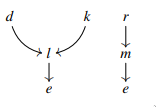
\includegraphics{assets/causal_g.png}
    \caption{Αιτιολογικός γράφος λογικού ποργράμματος (εξ. \ref{eq:example-cg}).}
    \label{fig:causal-g}
\end{figure}



Το εργαλείο \textit{xclingo}\footnote{\url{https://github.com/bramucas/xclingo2}} \cite{Cabalar_2020} επιτρέπει την παρουσίαση αιτιολογήσεων σχετικά με τα αποτελέσματα που δίνονται από τον επιλυτή \textit{Clingo}.
Αυτό επιτυγχάνεται προσθέτοντας ένα \src{trace} που αντιστοιχεί στους κανόνες του λογικού προγράμματός μας.
Η παροχή μιας σαφούς εξηγήσεως για το πώς το σύστημα κατέληξε σε συγκεκριμένα συμπεράσματα, μπορεί να βοηθήσει στον εντοπισμό πιθανών σφαλμάτων κατά την δημιουργία της βάσης γνώσης και να παρέχει στον χρήστη του συστήματος μια αιτιολόγηση για το τελικό αποτέλεσμα. Αυτό είναι κάτι πολύ σημαντικό στην περίπτωση που η εφαρμογή χρησιμοποιείται σε ιατρικά πλαίσια.

\section{Αποτελέσματα}

Για την αξιολόγηση του συστήματός μας χρησιμοποίησαμε δημοσίως διαθέσιμα δεδομένα ασθενών\footnote{\url{https://www.kaggle.com/datasets/itachi9604/disease-symptom-description-dataset?select=dataset.csv}}.
Στο σύστημά μπήκε σαν είσοδος το σύνολο των συμπτωμάτων του κάθε ασθενή.
Σαν βάση γνώσης έχουμε τον συνδυασμό όλων των κανόνων που έχουν προκύψει από την κωδικοποίηση την ιατρικής βιβλιογραφίας.  
Μία επιτυχημένη πρόβλεψη ορίζεται όταν η πραγματική ασθένεια του ασθενή συμπίπτει με την τελική
πρόβλεψη του επιλυτή ASP.

\begin{table}[h]
    \centering
    \begin{tabular}{lcc}
    \hline
    Ασθένεις & Μέγεθος Βάσης Γνώσης & Ακρίβεια \\
    \hline
    \hline
    Chicken Pox      &  66  & 95\% \\
    Pneumonia        &  75  & 100\% \\
    Common Cold    &   44 & 100\% \\
    \hline
    \end{tabular}
    \caption{Ακρίβεια της μεθόδου για μερικές ενδεικτικές ασθένειες.}
\end{table}

Η ακρίβεια του μοντέλου μας μπορεί να φτάσει πολύ υψηλά ποσοστά ακρίβειας αλλά απαιτεί την εισαγωγή ενός μεγάλου πλήθους κανόνων στη βάση γνώσης.
Το μέγεθος της βάσης γνώσης το ορίζουμε ως το πλήθος των λογικών όρων μέσα 
στο ASP πρόγραμμα που αντιστοιχεί σε κάθε μία από τις ασθένειες.

Στο πρόγραμμα που κατασκευάσαμε προσθέσαμε και τη δυνατότητα 
επεξήγησης της διάγνωσης, κατά την οποία αξιοποιούμε 
το εργαλείο \src{xclingo} για τη δημιουργία ενός γραφήματος
το οποίο αποτυπώνει τους συνειρμούς που ακολούθησε το σύστημά 
μας για τις προβλέψεις του.

\begin{lstlisting}[caption={Μέρος της επεξήγησης για τη διάγνωση της ασθένειας chickenpox. Μέσα στο διάγραμμα δέντρο φαίνονται οι συσχετίσεις μεταξύ των διαφορετικών συμπτωμάτων 
και το πώς το σύστημά μας καταλήγει στα συμπεράσματά του.}, label=lst:terms]{Name}
  *
  |__diagnosis(chickenpox)
  |  |__has(symptom(itching));has(symptom(itching))
  |  |__has(symptom(fatigue));has(symptom(fatigue));has(symptom(fatigue));has(symptom(fatigue));has(symptom(fatigue))
  |  |__has(symptom(lethargy))
  |  |  |__has(symptom(fatigue));has(symptom(fatigue));has(symptom(fatigue));has(symptom(fatigue));has(symptom(fatigue))
  |  |  |__linked_symptom(fatigue,lethargy)
  |  |__has(symptom(high_fever))
  |  |  |__has(symptom(mild_fever));has(symptom(mild_fever))
  |  |  |  |__has(symptom(loss_of_appetite));has(symptom(loss_of_appetite))
  |  |  |  |__linked_symptom(loss_of_appetite,mild_fever)
  |  |  |__linked_symptom(mild_fever,high_fever)
  |  |__has(symptom(loss_of_appetite));has(symptom(loss_of_appetite))
  |  |__has(symptom(mild_fever));has(symptom(mild_fever))
  |  |  |__has(symptom(loss_of_appetite));has(symptom(loss_of_appetite))
  |  |  |__linked_symptom(loss_of_appetite,mild_fever)
  |  |__has(symptom(swelled_lymph_nodes))
  |  |  
  ...
\end{lstlisting}

\section{Συμπεράσματα}

Στην εργασία αυτή έγινε η παρουσίαση μίας μεθοδολογίας για την αυτόματη πρόβλεψη ασθενειών 
η οποία περιλαμβάνει την κωδικοποίηση ιατρικής βιβλιογραφίας και τη μετατροπή της σε κώδικα 
ASP μέσω ενός μεγάλου γλωσσικού μοντέλου.
Έγινε παρουσίαση του τρόπου λειτουργίας των μεγάλων γλωσσικών μοντέλων και του ASP, 
ενώ έγινε συγκεκριμένη αναφορά στο ρόλο που παίζει η κάθε τεχνολογία στο τελικό σύστημα.
Ακόμα, δείξαμε την αρχιτεκτονική μας και το πώς αυτές οι τεχνολογίες θα συνδυαστούν ενώ
δώσαμε συγκεκριμένες υλοποιητικές λεπτομέρειες τις οποίες αναπτύξαμε τόσο
για την δημιουργία ποιοτικών prompts για το μεγάλο γλωσσικό μοντέλο, όσο και
στην δομή των κανόνων στην τελική ASP βάση γνώσης.
Τελικά, εκτελέσαμε προβλέψεις πάνω σε ορισμένες ασθένειες για τις οποίες δημιουργήσαμε την
βάση γνώσης με τη χρήση της μεθοδολογίας μας και παρουσιάσαμε τα αποτελέσματα.
Η μέθοδός μας φαίνεται να έχει υποσχόμενα αποτελέσματα και προσφέρει αξιόπιστες προβλέψεις υψηλής ακρίβειας
μαζί με τις επεξηγήσεις τους.

Μελλοντική δουλειά είναι η επέκταση της μεθόδου για περισσότερες ασθένειες.
Ταυτόχρονα θα ήταν χρήσιμη η δημιουργία μίας γραφικής διεπαφής μέσω 
της οποίας κάποιος να μπορεί να εισάγει στοιχεία κάποιου ασθενή και να παίρνει 
πιθανές διαγνώσεις.

\newpage
\bibliographystyle{unsrt}
\bibliography{bibliography}

\end{document}
